This section provides the exact derivation of the \gls{bearing-angle} formula.
The literature on \gls{bearing-angle} disagrees on the formula and have mathematical errors.
The full chain of derivation and graphical presentations goal is to provide a trustworthy and checkable background for the provided formula.

\begin{figure}[H]
    \tikzset{every picture/.style={line width=0.75pt}} %set default line width to 0.75pt        
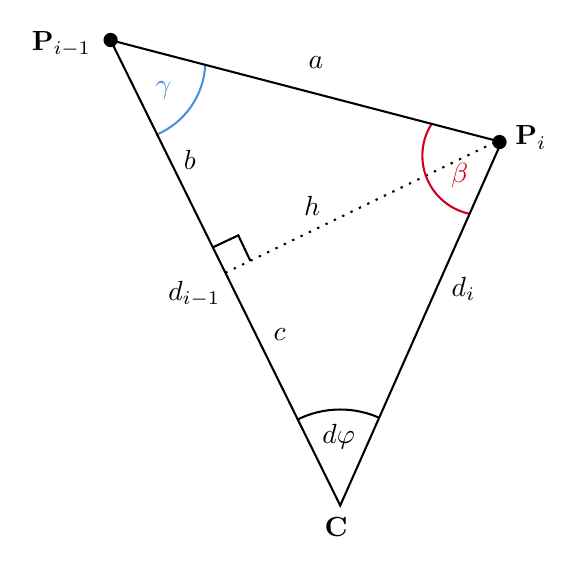
\begin{tikzpicture}[x=0.75pt,y=0.75pt,yscale=-1,xscale=1]
    %uncomment if require: \path (0,341); %set diagram left start at 0, and has height of 341

    %Straight Lines [id:da6739847496898159] 
    \draw  [dash pattern={on 0.84pt off 2.51pt}]  (122.83,145.01) -- (252.88,82) ;
    %Shape: Arc [id:dp4878212457791631] 
    \draw  [draw opacity=0] (240.62,116.61) .. controls (227.55,113.98) and (217.71,102.44) .. (217.71,88.6) .. controls (217.71,82.88) and (219.39,77.55) .. (222.28,73.08) -- (246.29,88.6) -- cycle ; \draw  [color={rgb, 255:red, 208; green, 2; blue, 27 }  ,draw opacity=1 ] (240.62,116.61) .. controls (227.55,113.98) and (217.71,102.44) .. (217.71,88.6) .. controls (217.71,82.88) and (219.39,77.55) .. (222.28,73.08) ;
    %Shape: Arc [id:dp901574933751006] 
    \draw  [draw opacity=0] (113.13,44.58) .. controls (112.48,59.91) and (102.88,72.93) .. (89.43,78.54) -- (74.58,42.92) -- cycle ; \draw  [color={rgb, 255:red, 74; green, 144; blue, 226 }  ,draw opacity=1 ] (113.13,44.58) .. controls (112.48,59.91) and (102.88,72.93) .. (89.43,78.54) ;
    %Shape: Polygon [id:ds6190617836836185] 
    \draw   (67.51,32.91) -- (255.81,82) -- (178.15,257.12) -- cycle ;
    %Shape: Ellipse [id:dp4849771561113211] 
    \draw  [fill={rgb, 255:red, 0; green, 0; blue, 0 }  ,fill opacity=1 ] (251.95,82) .. controls (251.95,80.38) and (253.26,79.07) .. (254.88,79.07) .. controls (256.5,79.07) and (257.81,80.38) .. (257.81,82) .. controls (257.81,83.62) and (256.5,84.93) .. (254.88,84.93) .. controls (253.26,84.93) and (251.95,83.62) .. (251.95,82) -- cycle ;
    %Shape: Circle [id:dp8356396848663105] 
    \draw  [fill={rgb, 255:red, 0; green, 0; blue, 0 }  ,fill opacity=1 ] (64.58,32.84) .. controls (64.58,31.22) and (65.89,29.91) .. (67.51,29.91) .. controls (69.13,29.91) and (70.44,31.22) .. (70.44,32.84) .. controls (70.44,34.46) and (69.13,35.77) .. (67.51,35.77) .. controls (65.89,35.77) and (64.58,34.46) .. (64.58,32.84) -- cycle ;
    %Shape: Arc [id:dp8012007227541399] 
    \draw  [draw opacity=0] (157.23,215.86) .. controls (163.51,212.67) and (170.62,210.87) .. (178.15,210.87) .. controls (184.79,210.87) and (191.12,212.27) .. (196.83,214.8) -- (178.15,257.12) -- cycle ; \draw   (157.23,215.86) .. controls (163.51,212.67) and (170.62,210.87) .. (178.15,210.87) .. controls (184.79,210.87) and (191.12,212.27) .. (196.83,214.8) ;
    %Shape: Right Angle [id:dp07010543377164635] 
    \draw   (116.98,132.65) -- (129.04,126.95) -- (134.88,139.31) ;

    % Text Node
    \draw (161.42,39.19) node [anchor=north west][inner sep=0.75pt]   [align=left] {$\displaystyle a$};
    % Text Node
    \draw (159.22,106.59) node [anchor=north west][inner sep=0.75pt]   [align=left] {$\displaystyle h$};
    % Text Node
    \draw (230.37,145.44) node [anchor=north west][inner sep=0.75pt]   [align=left] {$\displaystyle d_{i}$};
    % Text Node
    \draw (93.81,147.37) node [anchor=north west][inner sep=0.75pt]   [align=left] {$\displaystyle d_{i-1}$};
    % Text Node
    \draw (168.08,216.65) node [anchor=north west][inner sep=0.75pt]   [align=left] {$\displaystyle d\varphi $};
    % Text Node
    \draw (230.1,90.96) node [anchor=north west][inner sep=0.75pt]  [color={rgb, 255:red, 208; green, 2; blue, 27 }  ,opacity=1 ] [align=left] {$\displaystyle \beta $};
    % Text Node
    \draw (87.69,51.2) node [anchor=north west][inner sep=0.75pt]  [color={rgb, 255:red, 74; green, 144; blue, 226 }  ,opacity=1 ] [align=left] {$\displaystyle \gamma $};
    % Text Node
    \draw (101.34,84.61) node [anchor=north west][inner sep=0.75pt]   [align=left] {$\displaystyle b$};
    % Text Node
    \draw (144.57,170.34) node [anchor=north west][inner sep=0.75pt]   [align=left] {$\displaystyle c$};
    % Text Node
    \draw (169.08,261.2) node [anchor=north west][inner sep=0.75pt]   [align=left] {$\displaystyle \mathbf{C}$};
    % Text Node
    \draw (261,72.76) node [anchor=north west][inner sep=0.75pt]   [align=left] {$\displaystyle \mathbf{P}_{i}$};
    % Text Node
    \draw (28.06,27.4) node [anchor=north west][inner sep=0.75pt]   [align=left] {$\displaystyle \mathbf{P}_{i-1}$};
\end{tikzpicture}

    \caption[Derivation of the \gls{bearing-angle} with all support variables]{\emph{Derivation of the \gls{bearing-angle} with all support variables.} Deriving the bearing angle requires additional support variables that are introduced with this figure. Using fundamental trigonometry allows derivation of the formula.}\label{fig:bearing-derivation}
\end{figure}

The cosine theorem holds true for all triangles and is the central equality for the derivation.
\begin{equation}
\begin{aligned}
    \text{Ansatz:} \\
    d_{i-1}^2 &= d_i^2 + a^2 - 2 d_i a \cos \beta \qquad \text{(Cosine Theorem)} \\
\end{aligned}
\end{equation}
Introducing supporting variables at the positions given in Figure~\ref{fig:bearing-derivation} allows substituting the missing quantity $a$.
\begin{equation}
\begin{aligned}
    h &= d_i \sin d\varphi \\
    c &= d_i \cos d\varphi \\
    b &= d_{i-1} - d_i \cos d\varphi \\
    a^2 &= h^2 + b^2 \\
    a^2 &= \mathunderline{darkgreen}{(d_i \sin d\varphi)^2} + \mathunderline{plotblue}{(d_{i-1} - d_i \cos d\varphi)^2} \\
    a^2 &= \mathunderline{darkgreen}{\mathunderline{darkred}{d_i^2 \sin^2 d\varphi}} +
           \mathunderline{plotblue}{%
             \mathunderline{plotorange}{d_{i-1}^2 - 2 d_{i-1} d_i \cos d\varphi} +
             \mathunderline{darkred}{d_i^2 \cos^2 d\varphi}
           } \\
    a^2 &= \mathunderline{darkred}{d_{i-1}^2 \sin^2 d\varphi + d_{i-i}^2 \cos^2 d\varphi} +
           \mathunderline{plotorange}{d_{i-1}^2 -2 d_{i-1} d_i \cos d\varphi} \\
    a^2 &= \mathunderline{darkred}{d_i^2} +
           \mathunderline{plotorange}{d_{i-1}^2 - 2 d_{i-1} d_i \cos d\varphi} \\
\end{aligned}
\end{equation}
For $a$ holds the condition $a > 0$ for all values, because the constraints $d_i > 0$, $d_{i-1} > 0$ and $0 < d\varphi < \pi$ result from the properties of depth sensors.

The variable $a$ is now substituted in the ansatz.
Consequent simplification of the equations yields the final formula for the bearing angle.
\begin{equation}
\begin{aligned}
    d_{i-1}^2 &= d_i^2 + a^2 - 2 d_i a \cos \beta \\
    \mathunderline{plotblue}{d_{i-1}^2} &= \mathunderline{darkred}{d_i^2} +
    \mathunderline{darkred}{d_i^2} + \mathunderline{plotblue}{d_{i-1}^2} - 2 d_{i-1} d_i \cos d\varphi
    - 2 d_i \sqrt{d_i^2 + d_{i-1}^2 -2 d_{i-1} d_i \cos d\varphi} \cos \beta \\
    \mathunderline{plotblue}{0} &= \mathunderline{darkgreen}{2} \mathunderline{darkred}{d_i^2} +
                                   \mathunderline{plotblue}{0} -
                                   \mathunderline{darkgreen}{2} d_{i-1} \mathunderline{darkred}{d_i} \cos d\varphi
                                   - \mathunderline{darkgreen}{2} \mathunderline{darkred}{d_i} \sqrt{d_i^2 + d_{i-1}^2 -2 d_{i-1} d_i \cos d\varphi} \cos \beta \\
   0 &= \mathunderline{darkred}{d_i^2} - d_{i-1}\mathunderline{darkred}{d_{i}} \cos d\varphi
       - \mathunderline{darkred}{d_i} \sqrt{d_i^2 + d_{i-1}^2 -2 d_{i-1} d_i \cos d\varphi} \cos \beta \\
   0 &= \mathunderline{darkred}{d_i} - \mathunderline{darkred}{1} d_{i-1} \cos d\varphi
       - \mathunderline{darkred}{1} \sqrt{d_i^2 + d_{i-1}^2 -2 d_{i-1} d_i \cos d\varphi} \cos \beta \\
   \cos \beta &= \frac{d_i - d_{i-1} \cos d\varphi}{\sqrt{d_i^2 + d_{i-1}^2 -2 d_{i-1} d_i \cos d\varphi}} \\
   \beta &= \arccos \frac{d_i - d_{i-1} \cos d\varphi}{\sqrt{d_i^2 + d_{i-1}^2 -2 d_{i-1} d_i \cos d\varphi}} \\
\end{aligned}
\end{equation}

% vim: set nocindent nosmartindent
